\pdfoutput=1

\documentclass{l4proj}

\usepackage{hyperref}
\hypersetup{
	colorlinks=false,
    citebordercolor={0 1 0},
    filebordercolor={1 1 0},
    linkbordercolor={1 0 0},
    urlbordercolor={0 1 1}
}

\usepackage{chngcntr}
\counterwithout{figure}{chapter}

\begin{document}
\title{Exploring the possibility of accelerating Hurricane Simulator using Apache Spark framework}
\author{Andrej Hoos}
%\date{March ???, 2016}
\maketitle

\begin{abstract}
The bestest abstract
\end{abstract}

\educationalconsent
%
%NOTE: if you include the educationalconsent (above) and your project is graded an A then
%      it may be entered in the CS Hall of Fame
%
\tableofcontents
%==============================================================================

%==============================================================================
%  Introduction
%==============================================================================
\chapter{Introduction}
\pagenumbering{arabic}

Simulating real world weather system is a difficult task, requiring a lot of computational power.
One such simulator is The Large Eddy Simulator for the Study of Urban Boundary-layer Flows (LES)
developed by  Hiromasa Nakayama and Haruyasu Nagai at the Japan Atomic Energy Agency
and Prof. Tetsuya Takemi at the Disaster Prevention Research Institute of Kyoto University\cite{les_analysis}\cite{les}.
It simulates meteorological systems in an urban environment with building resolution.
Originally LES is implemented in Fortran 77 with no explicit parallelization.

\section{Motivation \& Aim}

As multi core computational devices are now commonplace, parallelisation has become
a important consideration when implementing simulations. Therefore LES has been
ported to Fortran 95/OpenCL implementation by Wim Vanderbauwhed\cite{les_wim}. Using this implementation,
LES can be run parallelised on any OpenCL compatible computational device, which shows
significant improvements in speed. While these improvements can reduce the time needed to
run single simulation run or increase the size of the spatial domain of the simulation,
there are limits to both. One of these limits is number of computational units the device has,
limiting the extent of parallelization. The other is memory available on the device.

Using a network cluster of computers can, in theory, help overcome these limits to some extent.
However, splitting work onto multiple nodes in a cluster introduces a issue of communicating
important information over network. Specifically, in case of LES, data that is at the edge of
the spatial domain of each node needs to be exchanged in so called halo exchanges.

Recently, there has been a rise in a new computational frameworks focused on working in
distributed environment. One of these frameworks is Apache Spark which is based on
the MapReduce parallel execution paradigm.

The aim of this report is to explore the possibility of using the Apache Spark in Java to parallelize
LES, or any algorithm relying on halo exchanges in network distributed environment.

\section{Outline}

Further background will be described in \autoref{chap:background}, including information
on LES, Apache Spark and OpenCL implementation used. Implementation of halo exchanges in 
Apache Spark will be discussed in \autoref{chap:halos} and \autoref{chap:les_java} will
explain the process of porting LES code from Fortran to Java. Evaluation of the achieved
performance can be found in \autoref{chap:eval} and \autoref{chap:conclusion} contains
final remarks and notes about future work.

%==============================================================================
%  Background
%==============================================================================
\chapter{Background}
\label{chap:background}

\section{Large Eddy Simulator}

The Large Eddy Simulator for the Study of Urban Boundary-layer Flows developed by
Disaster Prevention Research Institute of Kyoto University is a high resolution
meteorological simulator designed to model turbulent flows over urban topologies. 
It achieves this by using mesoscale meteorological simulations and building resolving
large-eddy simulations. It also uses The Weather Research and Forecasting Model \footnote{\url{http://www.wrf-model.org}}
to compute the wind proile as an input for the simulation. The simulation is split into
multiple subroutines, however, the most important one is the Poisson Equation solver.
This is the most computationally intensive subroutine and it uses successive over relaxation to solve
a linear system of equations. Each time step of the simulation needs to execute following subroutines
in a sequence:

\begin{tabular}{ | l | l | }
  \hline	
  \textbf{velnw} & Update velocity for current time step \\
  \textbf{bondv1} & Calculate boundary conditions (initial wind profile, inflow, outflow) \\
  \textbf{velfg} & Calculate the body force \\
  \textbf{feedbf} & Calculation of building effects \\
  \textbf{les} & Calculation of viscosity terms (Smagorinsky model) \\
  \textbf{adam} & Adams-Bashforth time integration \\
  \textbf{press} & Solving of Poisson equation (SOR) \\
  \hline	
\end{tabular}

LES runs over spatial domain represent by a 3D grid. Size of 150x150x90 is used	for the most
of this report, but the size can be varied in x and y direction. By increasing the size of the
grid in x and y directions, LES can be run with higher resulution, or it can used 
to cover larger area. However doing this increases the time needed to complete the simulation
and more importantly there is a limit to how big the grid can be so that it fits inside the RAM.

\subsection{Paralellisation}

Using a cluster of computers, we can split the domain such that every node in the cluster runs
LES on a small portion of the domain. This allows to run LES on much larger domain than what would be
possible on a single computer. To run LES correctly in this scenario, each node needs access to the 
edge data belonging to each of its eight neighbours (Figure \ref{fig:neighbours}).

\begin{figure}
\centering
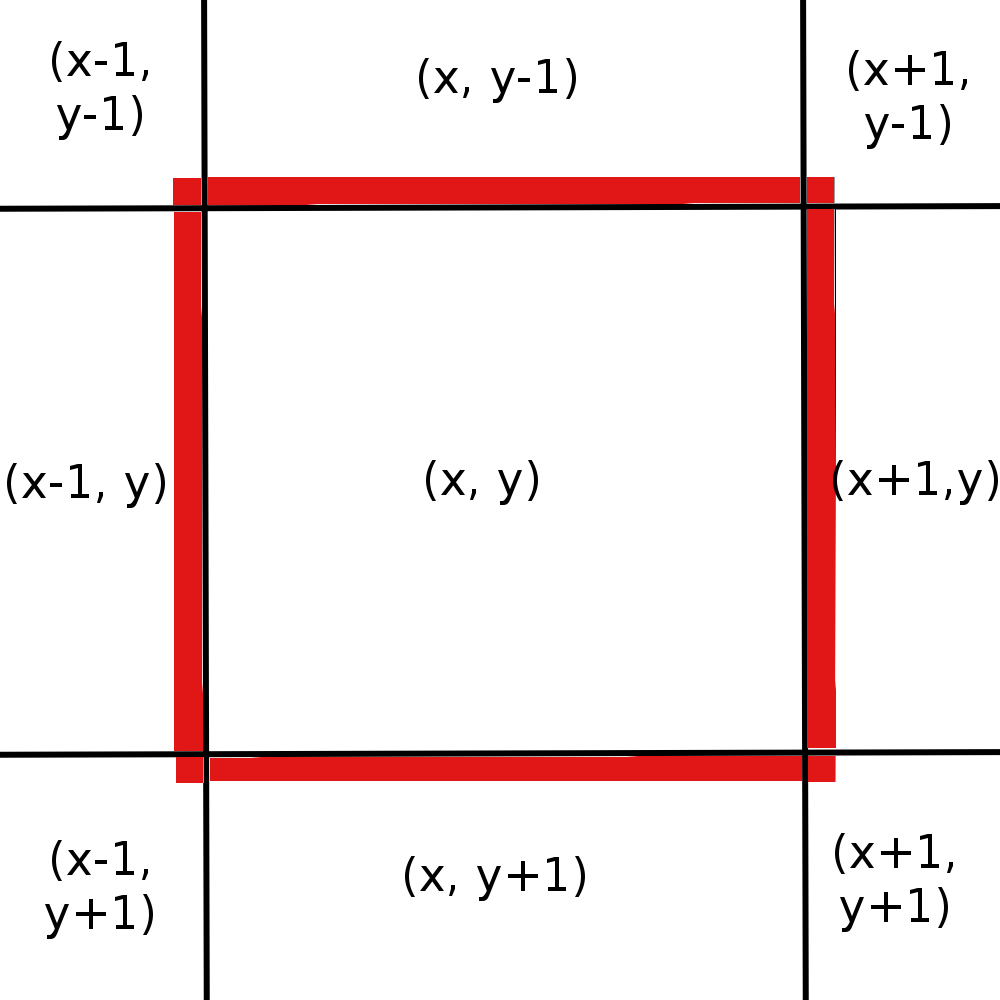
\includegraphics[width=0.5\textwidth]{images/neighbours.png}
\caption{Node (x,y) needs access to the edges of all its neighbours}
\label{fig:neighbours}
\end{figure}

Message Passing Interface (MPI) \footnote{\url{http://www.mcs.anl.gov/research/projects/mpi/mpi-standard/mpi-report-2.0/mpi2-report.htm}} 
is considered to be most commonly used for communication in distributed memory environments.
Because of this, LES has already been parallelised using MPI by Gordon Reid as his MSci project at University of Glasgow\cite{les_mpi} and others\cite{les_palm}. Although MPI is considered standard and achieves good performance, it
isn't easy task to parallelise algorithms using MPI, especially for scientists with minimal
experience with Computing Science. Therefore it is important to investigate the possibilty
of using frameworks with higher level abstraction and that are easy to deploy onto a standard
network cluster.


\section{MapReduce parallel processing}

MapReduce is a programming model used mainly for processing large quantities of data
and is intended for network clusters\cite{map_reduce}. Program using this model consists of Map and Reduces
methods which are automatically paralellised. MapReduce was originally name of a technology by
Google, but is now used for the model in general. MapReduce libraries and frameworks are now 
available in many programming languages.

MapReduce model usually operates on key-value pairs and can be described by three main steps:

\begin{itemize}  
\item \textbf{Map}: \textbf{map()} function is applied to all of the pairs, creating a collection of new key-value pairs
\item \textbf{Shuffle}: the output data is redistributed accross network such that pairs with the same key are located on the same node
\item \textbf{Reduce}: the output data is processed by applying the \textbf{reduce()} function to the output pairs
\end{itemize}

Advantage of using MapReduce is that only map() and reduce() functions need to be written and
the shuffle step is handled automatically by the library or framework and is usually optimised. 
In addition, most MapReduce frameworks provided more data manipulation methods such as grouping or 
joining.

\subsection{Apache Spark}

Apache Spark\footnote{\url{http://spark.apache.org/}} is one of these frameworks and is available Java, Scala, Python and R. It claims
to be faster over alternatives such as Apache Hadoop, because it allows MapReduce to run in
memory as opposed to reading and writing inputs and outpus solely from disk. This, with combination
that is the increasing community and high-level abstraction makes this framework suitable for the purposes
of this project.	

TODO: Describe main points about how Spark works (master, worker, driver, RDDs...)

\section{OpenCL}

TODO: OpenCL background\footnote{\url{https://www.khronos.org/opencl/}}
\subsection{Aparapi}
TODO: Aparapi background
\footnote{\url{http://developer.amd.com/tools-and-sdks/opencl-zone/aparapi/}}
\footnote{\url{https://aparapi.github.io/}}

%==============================================================================
%  Halo exchanges in Spark
%==============================================================================
\chapter{Halo exchanges in Spark}
\label{chap:halos}

The main challenge of this project is to construct viable halo exchange algorithm, using 
data manipulation methods provided by Apache Spark. This has not been done before, although
one work\cite{seismic_spark} has used Spark to solve a stencil problem computation. In stencil
problems, the problem is divided into cells, and to compute one cell, information about its
neighbours are needed. However, only simple method using broadcast variables (covered later in the chapter)
was used in this work.

Multiple possible algorithms were considered and their implementation details, advantages
and drawbacks are discussed in this chapter.

\section{Game of Life as a proof of concept}
To test the proposed alorithms, a implemetation of Conway's Game of Life was used.
This was because of its simplicity and becasue it resembles the simulator in that
in needs data from neighbours to be transfered in order to be parallelised in 
distributed environment.

The Game of Life is a cellular automaton and is run on a 2D grid of cells. To compute
the transition of a single cell, state of each of its eight neigbours are needed.
The transitions are defined as:

\begin{itemize} 
\item Any live cell with fewer than two live neighbours dies.
\item Any live cell with two or three live neighbours lives on to the next generation.
\item Any live cell with more than three live neighbours dies.
\item Any dead cell with exactly three live neighbours becomes a live cell.
\end{itemize}

We can group the cells into same size rectangle shaped chunks and compute the transitions of each
chunk on a separate node of the cluster. However, now the nearest edges of neighbouring
chunks need to be exchanged before each transition, in order for the edge cells to know
the state of all of their neighbours. This is the same case in the LES and is therefore
suitable as a proof of concept.

\section{Broadcast variables}

The simplest way exchange halos is using broadcast variables. Spark allows to
create a broadcast variable in the driver program, which is the shipped to worker
nodes if needed. However the limitation is that only the driver program can create
broadcast variables (i.e. they cannot be created in the worker code) and therefore
the workers would need to send their edge data to the driver program, which would
contruct the appropriate halos and create a broadcast variable(TODO: diagram).

This means that the halos would be transferred to their destination always via
the node which hosts the driver program, and therefore the algorithm would do 
twice as much network transfers as the ideal case where the halos are transferred
to their destination directly. Therefore this approach was deemed unsuitable. 

\section{MapReduceByKey}

Another way is to use a combination of map and reduce steps (TODO: diagram). To represent the 
chunks, we use Spark Pair Collection of pairs of key and chunk (\texttt{JavaPairRDD<String, Chunk>}). The key represents
the coordinates of the chunk.

In the first stage we transform this collection into another collection which contains
the chunks from the original collection together with all neighbours using map
(\texttt{flatMapToPair}). The keys of the neighbours key value pairs are the keys of their respective
target chunk.

The second step then does reduce on this new collection using \texttt{reduceByKey}. 
The reducer function takes a chunk and a neighbour and reduces them into a chunk
with the neighbour added to it, which results in a collection of chunks which are
larger by one cell on each side.

The last step is a map step, which computes next transition on each chunk, returning
collection of transformed chunk which are the original size.

There are, however, some drawbacks to this approach. The first is, that we cannot
control the exact order in which these operations are executed. For example, Spark
might decide to execute the first map step on first two chunks (assuming there are more than two)
and run the reduce step on the results. Then, the first map step might be run on the rest
of the chunks. The second issue is that we cannot control, on which node is each step 
executed. This two issues result in all of the chunks and not only neighbours are
transferred over network, which is unacceptable for the purpouses of this project.

\section{MapGroupByKey}

To resolve one of the issues mentioned above, it is possible to replace the reduce
step with group step (TODO: diagram). This uses \texttt{groupByKey} to group chunk together with
neighbours that share the same key. The grouping function takes the chunk with
its neighbours and combines them into a single chunk, such that the result is the
same as after the reduce step in previous section.

Using this method the issue of the order of execution is solved, since the group
can be executed only after all of first map stage has been executed. The second issue
of not being able to control where is each stage executed still remains and therefore
the issue of transferring all chunk over network remains as well.

\section{MapCogroup}

Method described in this section was inspired by chapter 4 in \textit{Learning Spark}\cite{learning_spark}.
It uses custom partitioner and two separate collections for chunks and neighbours
to prevent Spark from moving chunks around the network. It uses combination
of map and cogroup steps.

The first map operates on the same key value pair collection as above. However,
now it transforms the collection into separate key value pair collection of neighbours,
instead of creating one mixed one as was done previously (TODO: diagram).

In second step, the \texttt{cogroup} transformation is very similar to the grouping transformation
from the MapGroupByKey method, with the difference that in this case it operates on two collections 
instead of one. The result is the same as in previous sections.

In addition, the collection containing chunks is partitioned using custom partitioner.
The partitioner takes the key, which represents coordinates and outputs index of node
on which the chunk should be physically present. Using this partitioner spark
shuffles only the other collection, which contains neighbour data, over network and
keeps the chunks collection in place.

\section{Caching and checkpointing}

Spark uses lazy execution when running programs stages. This means that transformation
on a collection are saved in its lineage are executed only after a call
that materialises the collection on the driver program is called on it. Examples of such calls are
\texttt{count} that returns the number of items in the collection, \texttt{collect}
which returns array of all items in the collection or \texttt{reduce}, which, as opposed
to \texttt{reduceByKey} reduces the collection into single item.

This introduces some issues. First issue is that often, when resolving stages that
do network shuffle, Spark executes the parent stages more than once. This is
considered standard Spark behaviour and is solved by caching the parent collection
using \texttt{cache} method, which also marks the collection to be explicitly reused
when executing, child stages. However, it was found that Spark keeps more cached collections
than necessary, and therefore workaround was devised. Using this workaround, first,
new collection is created, then cached and materialised using \texttt{count} and 
then \texttt{unpersist} is called on the old collection to remove it from the cache.

Another issue is lineage length. In iterative algorithms, such as the ones described 
in this report, the lineage that Spark keeps in order to be able to restore execution
in the case of failure can get quite long. This results in significant slowdown of
Spark task resolution and eventually leads to stack overflow errors. One possible
solution is to increase JVM maximum stack memory, but the standard practice is to
\texttt{chekpoint} collections. This serializes the collection to disk and forgets
its lineage. 

%==============================================================================
%  LES in Java
%==============================================================================
\chapter{LES in Java}
\label{chap:les_java}

\section{Aparapi for Unconventional Cores}

\begin{verbatim}
Aparapi-UCores: A High Level Programming Framework for Unconventional Cores
http://ieeexplore.ieee.org/xpl/articleDetails.jsp?reload=true&arnumber=7322440
https://gitlab.com/mora/aparapi-ucores
\end{verbatim}

\subsection{Device specific OpenCL binaries}

\begin{verbatim}
https://github.com/adikus/cl-compile
\end{verbatim}

\subsection{Memory alignment}

\section{JNA with Fortran}

\begin{verbatim}
http://www.javaforge.com/wiki/66061
\end{verbatim}

\section{LES in Apache Spark}

\subsection{Caching \& Checkpointing}

%==============================================================================
%  Evaluation
%==============================================================================
\chapter{Evaluation}
\label{chap:eval}

\section{Architecture}

\begin{verbatim}
http://ark.intel.com/products/75267/Intel-Xeon-Processor-E5-2640-v2-20M-Cache-2_00-GHz
\end{verbatim}

\section{Baseline tests}

\section{Spark tests - increasing domain size}

%==============================================================================
%  Conclusion
%==============================================================================
\chapter{Conclusion}
\label{chap:conclusion}

\section{Future Work}

\section{Summary}

%%%%%%%%%%%%%%%%
%              %
%  APPENDICES  %
%              %
%%%%%%%%%%%%%%%%
\begin{appendices}

\begin{verbatim}
https://github.com/adikus/hurricaneProject
\end{verbatim}

\end{appendices}

%%%%%%%%%%%%%%%%%%%%
%   BIBLIOGRAPHY   %
%%%%%%%%%%%%%%%%%%%%

\bibliographystyle{plain}
\bibliography{bib}	

%%%%%%%%%%%%%%%%%%%
%   ???????????   %
%%%%%%%%%%%%%%%%%%%
\begin{verbatim}
H. Nakayama, T. Takemi, H. Nagai, and E. Agency,
“Coupling of WRF and building-resolving urban CFD
models for analysis of strong winds over an urban
area,” 3rd International Workshop on Nonhydrostatic
Numerical Models, vol. 3, no. RIKEN AICS, Kobe,
Japan, 2014.
\end{verbatim}

\end{document}
